% !TeX program = lualatex
% Author         : Pedro Ferreira (up201806093@up.pt)
% Version        : 1.0
% Created on     : 12.08.2022
% Last Edited on : 14.08.2022
% Adapted from HSRM theme by Benjamin Weiss
% Copyright      : Copyright (c) 2013-2014 by Benjamin Weiss. All rights reserved.
% License        : This file may be distributed and/or modified under the
%                  GNU Public License.
% Description    : HSRM beamer theme demonstration. Also includes a short 
%                  Tutorial regarding the beamer class.



%%%%%%%%%%%%%%%%%%%%%%%%%%%%%%%%%%%%%%%%%%%%%%%%%%%%%%%%%%%%%%%%%%%%%%%%%%%
%                    !!! Compile with LuaLaTex !!!
%%%%%%%%%%%%%%%%%%%%%%%%%%%%%%%%%%%%%%%%%%%%%%%%%%%%%%%%%%%%%%%%%%%%%%%%%%%

\documentclass[compress,aspectratio=169]{beamer}
%--------------------------------------------------------------------------
% Common packages
%--------------------------------------------------------------------------
\usepackage[french]{babel}
\hypersetup{
pdftitle={Présentation de pré-étude},
pdfsubject={Pré-étude},
pdfauthor={Ali Zoubir},
pdfkeywords={Latex,Beamer}}

\usepackage{graphicx}
\usepackage{multicol}
\usepackage[export]{adjustbox}

% Advanced table functions
\usepackage{tabularx,ragged2e}
\usepackage{booktabs}
% Listings extension
\usepackage{listings}
\lstset{ %
language=[LaTeX]TeX,
basicstyle=\normalsize\ttfamily,
keywordstyle=,
numbers=left,
numberstyle=\tiny\ttfamily,
stepnumber=1,
showspaces=false,
showstringspaces=false,
showtabs=false,
breaklines=true,
frame=tb,
framerule=0.5pt,
tabsize=4,
framexleftmargin=0.5em,
framexrightmargin=0.5em,
xleftmargin=0.5em,
xrightmargin=0.5em
}

%--------------------------------------------------------------------------
% Load theme
%--------------------------------------------------------------------------
\usepackage{sleektheme/beamerthemesleek}
\usetheme[]{sleek}

\usepackage{sleektheme/dtklogos} % must be loaded after theme
\usepackage{tikz}
\usetikzlibrary{mindmap,backgrounds}

%--------------------------------------------------------------------------
% General presentation settings
%--------------------------------------------------------------------------
\title{Présentation étude}
\subtitle{Localisation sous-marine 2221 \\ {\small Système de logging pour algorithme de localisation sous-marine}}
\date{Dérnière MAJ: \today}
\author{Ali Zoubir}
\institute{ETML-ES\\ {\Medium Génie électrique}}

%--------------------------------------------------------------------------
% Notes settings
%--------------------------------------------------------------------------
\setbeameroption{show notes}

\begin{document}
%--------------------------------------------------------------------------
% Titlepage
%--------------------------------------------------------------------------

\maketitle

%\begin{frame}[plain]
%	\titlepage
%\end{frame}

%--------------------------------------------------------------------------
% Table of contents
%--------------------------------------------------------------------------
\section*{Structure}
\begin{frame}{Structure}
	% hideallsubsections is recommended for longer presentations
	\tableofcontents[hideallsubsections]
\end{frame}

%--------------------------------------------------------------------------
% Content
%--------------------------------------------------------------------------
\section{Introduction}

\begin{frame}{Introduction de l'étude}
	Voici les éléments développés lors de l'étude :\vspace{-4pt}
	
	\begin{block}{Documentation}
		Rédaction d'un rapport de projet.
	\end{block}\vspace{-2mm}

	\begin{block}{Conception}
		Diagrammes et description de fonctionnement plus pointus.
	\end{block}\vspace{-2mm}
	
	\begin{block}{Mécanique}
		Réflexions idées et perspectives quant à la mécanique du module.
	\end{block}\vspace{-2mm}

	\begin{block}{Schématique}
		Développement d'un schéma électrique complet avec hiérarchie de fichiers.
	\end{block}\vspace{-2mm}
	
\end{frame}

\begin{frame}{Vue d'ensemble du système}
	\begin{figure}
		\par
		\noindent
		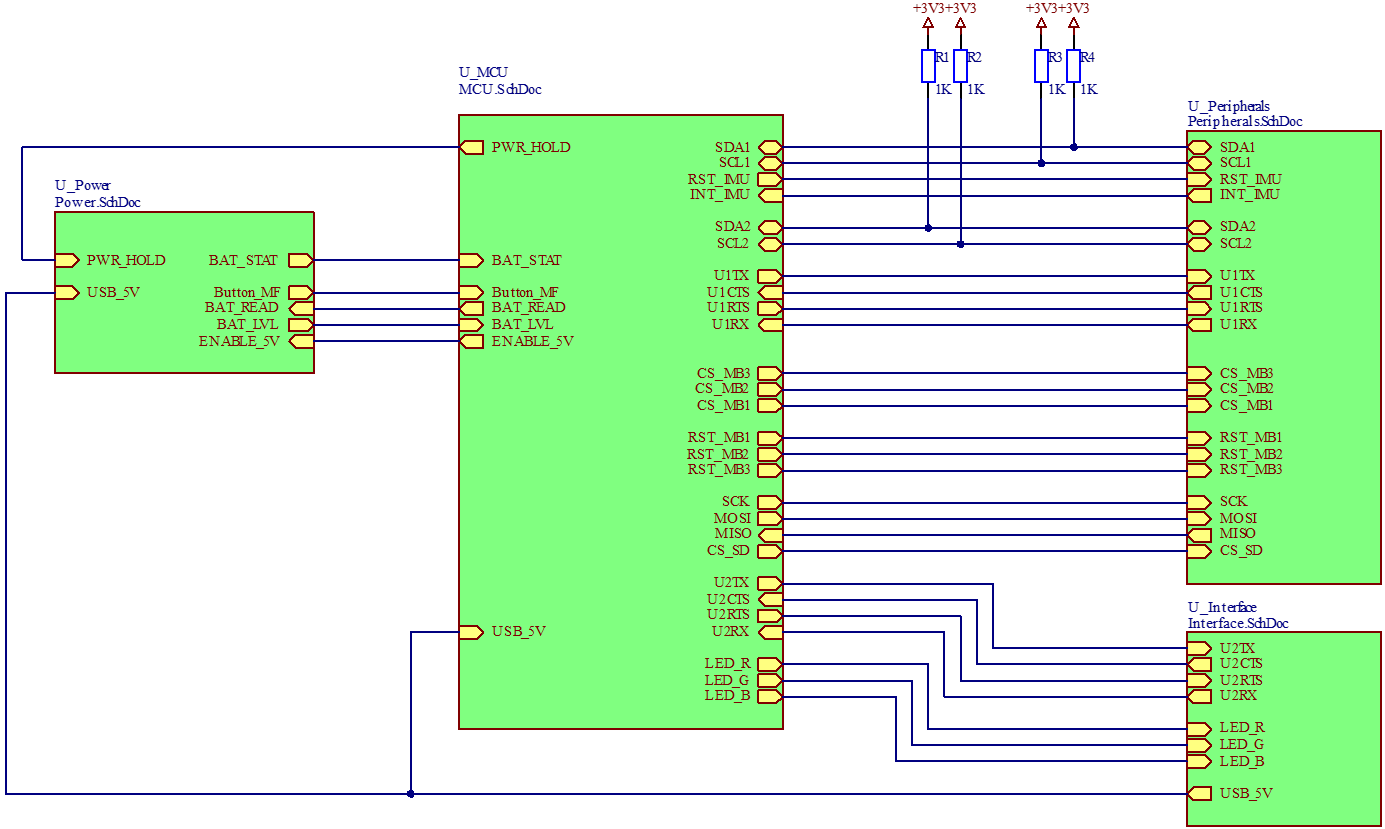
\includegraphics[width=0.55\linewidth]{Images/Dev-SCH/schemaBloc}%
		\hfill
		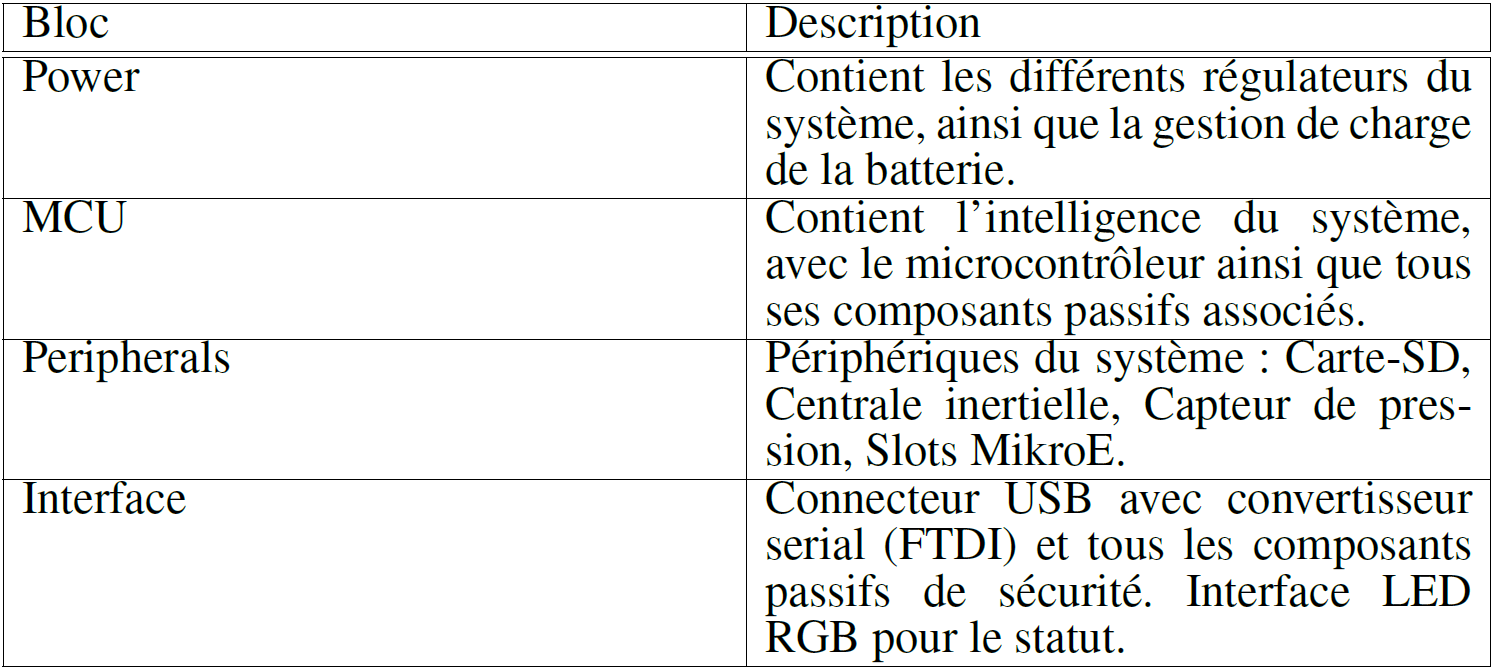
\includegraphics[width=0.45\linewidth]{Images/Dev-SCH/DescrBlocs}%
		\par
		\caption{Schéma bloc du système à jour}
	\end{figure}
\end{frame}

\section{Conception}

\begin{frame}[containsverbatim]{Consommation du système}
	\begin{center}
		\fbox{\textit{MCU - 30mA}} \fbox{\textit{BNO055 - 12.3mA}} \fbox{\textit{Capt. Pression - 4mA}} \fbox{\textit{\textcolor{red}{Carte-SD - 100mA}}} \fbox{\textit{MikroE - ??mA}} \fbox{\textit{Régulateurs - 40uA}} \fbox{\textit{LED RGB - 25mA}} 
	\end{center}
	\textbf{Total : 171,34mA}

	\begin{equation}
		Capacite = Consommation_{tot} * Temps
	\end{equation}
	
	\textbf{Pour 1 expédition (2h) : $\sim$342.68mAh}
	
	\textbf{Accu 3400mAh (Commande commune) : $\sim$20h}
	
	C’est un temps largement suffisant pour la durée de plusieurs expéditions,
	néanmoins la RTCC du microcontrôleur requiert d’être alimentée
	en permanence, un mécanisme de veille doit donc être mis en place.
\end{frame}

\begin{frame}[containsverbatim]{Concept fonctionnement}
	\begin{figure}
		\centering
		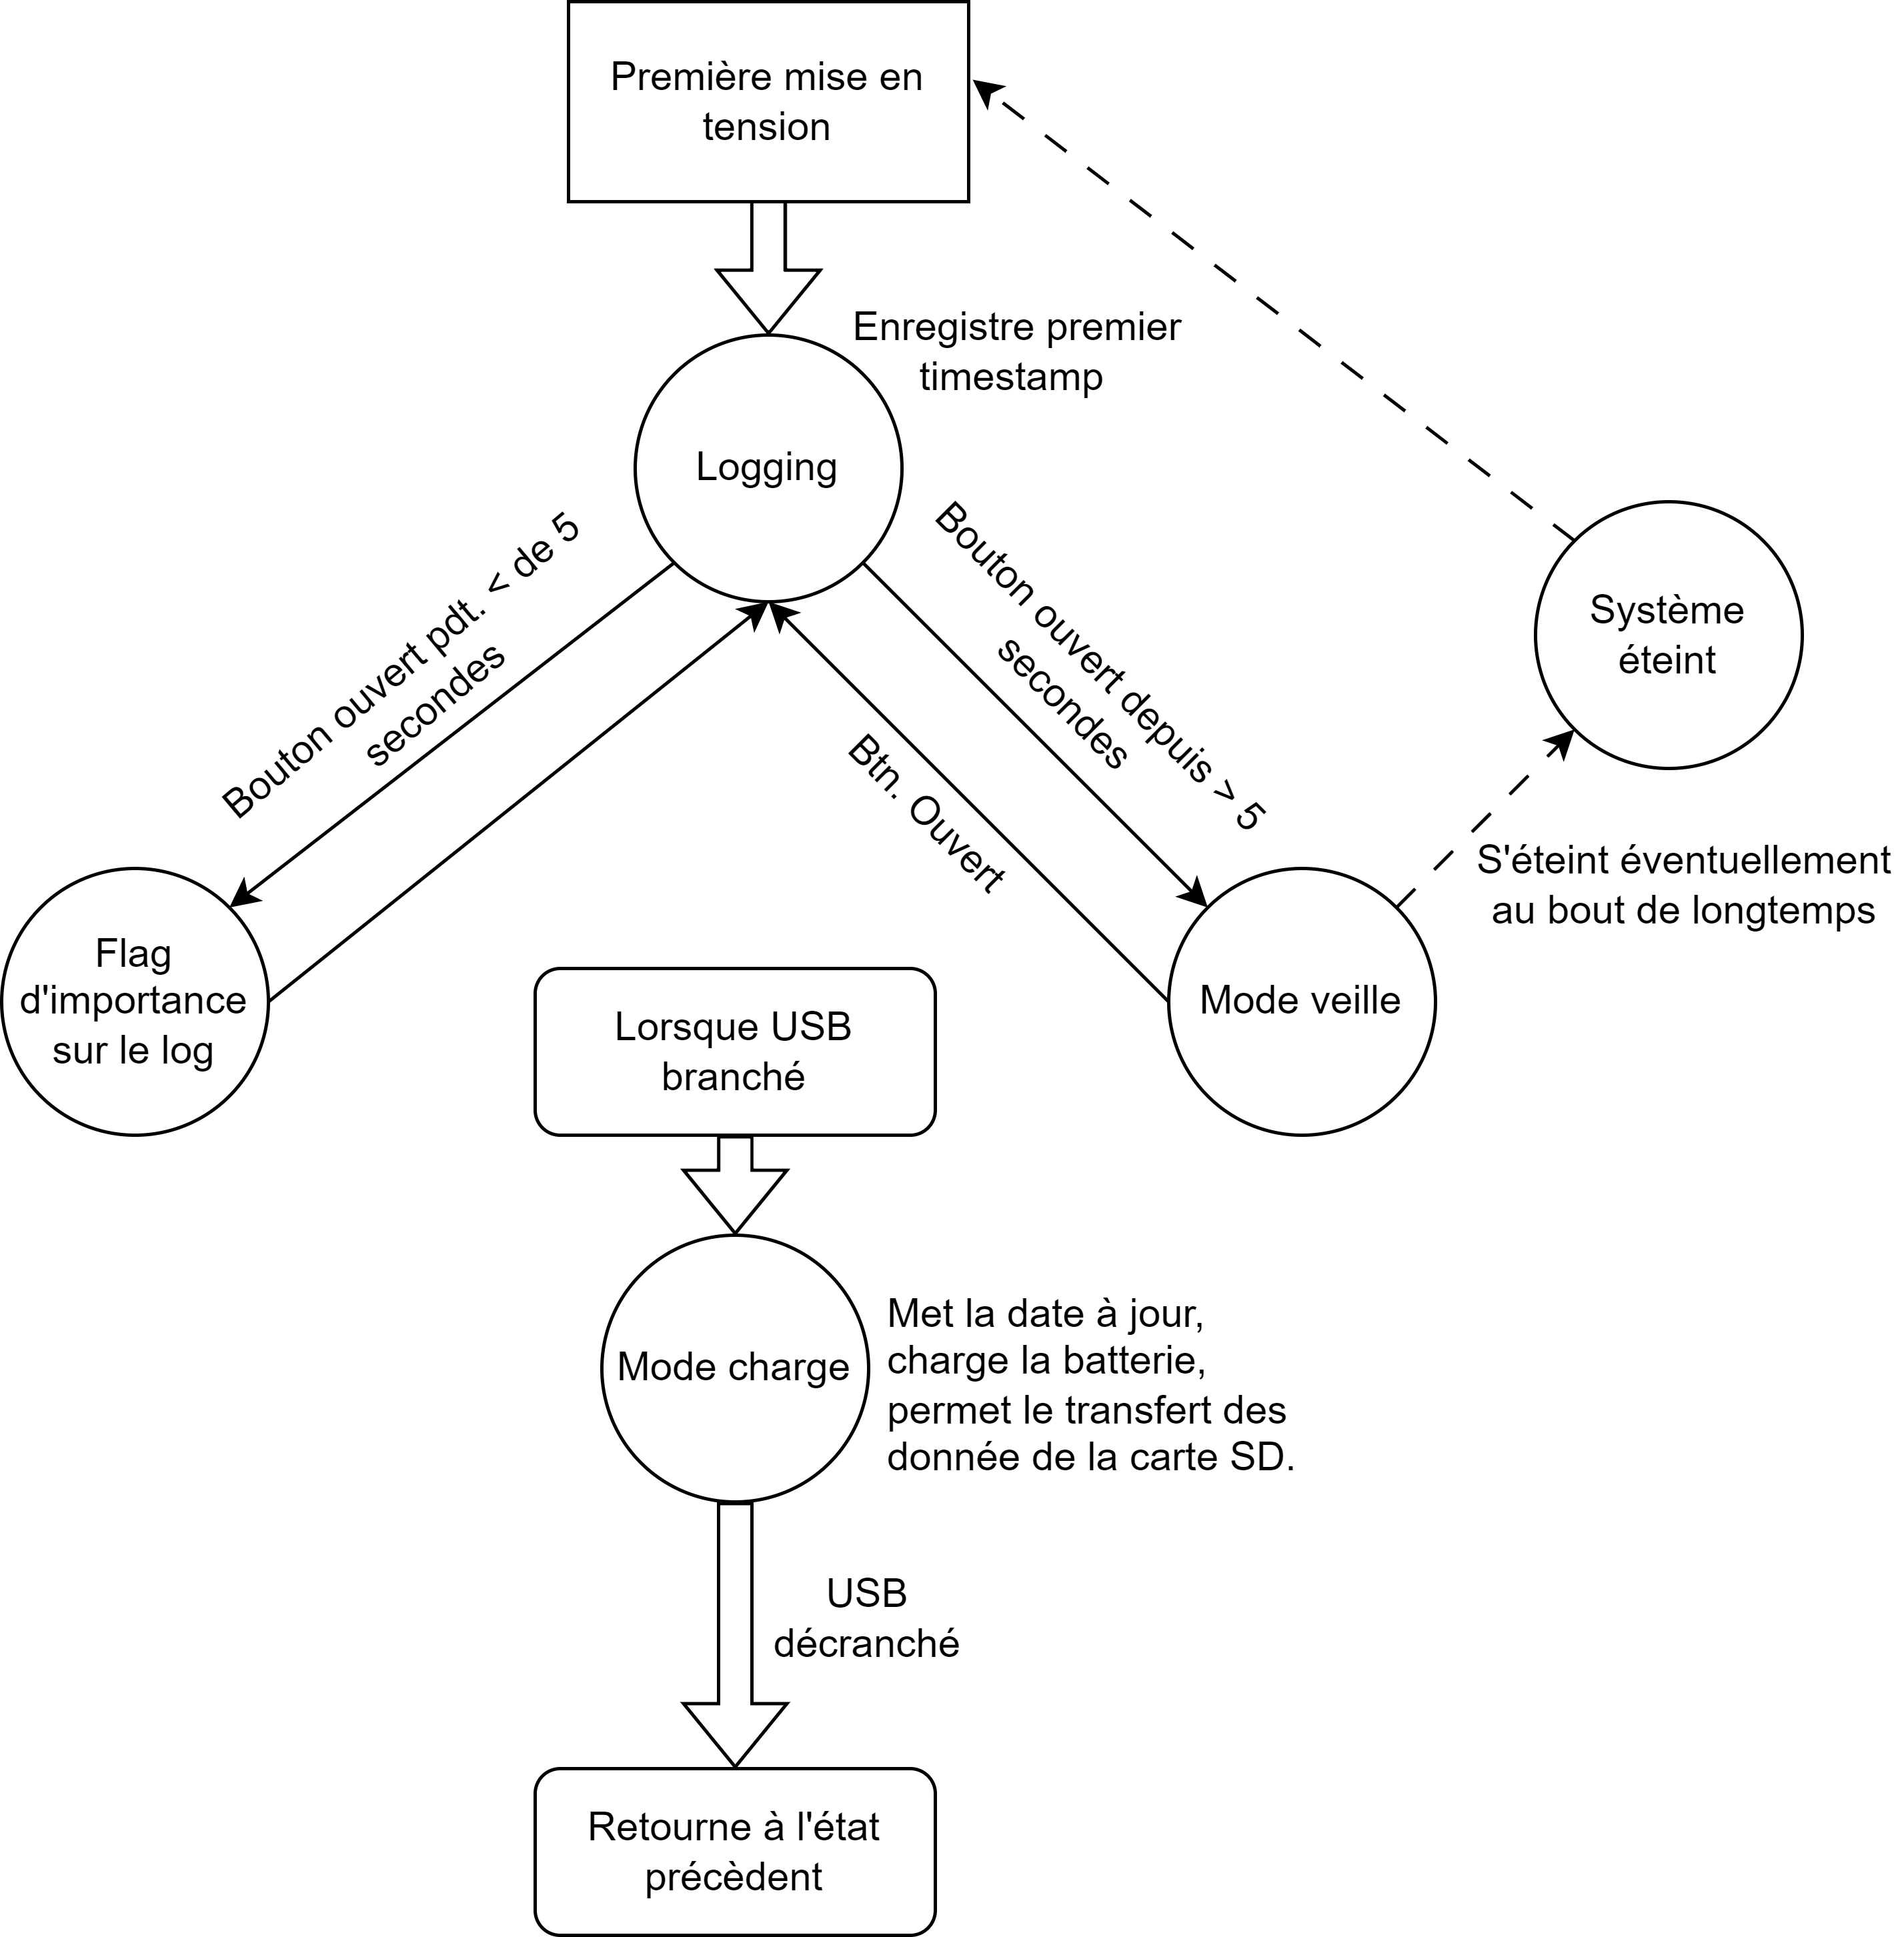
\includegraphics[width=0.5\linewidth]{Images/Dev-SCH/Etats_diagramme}
		\caption{Diagramme des états}
		\label{fig:etatsdiagramme}
	\end{figure}
\end{frame}
 
\begin{frame}
	\begin{figure}
		\centering
		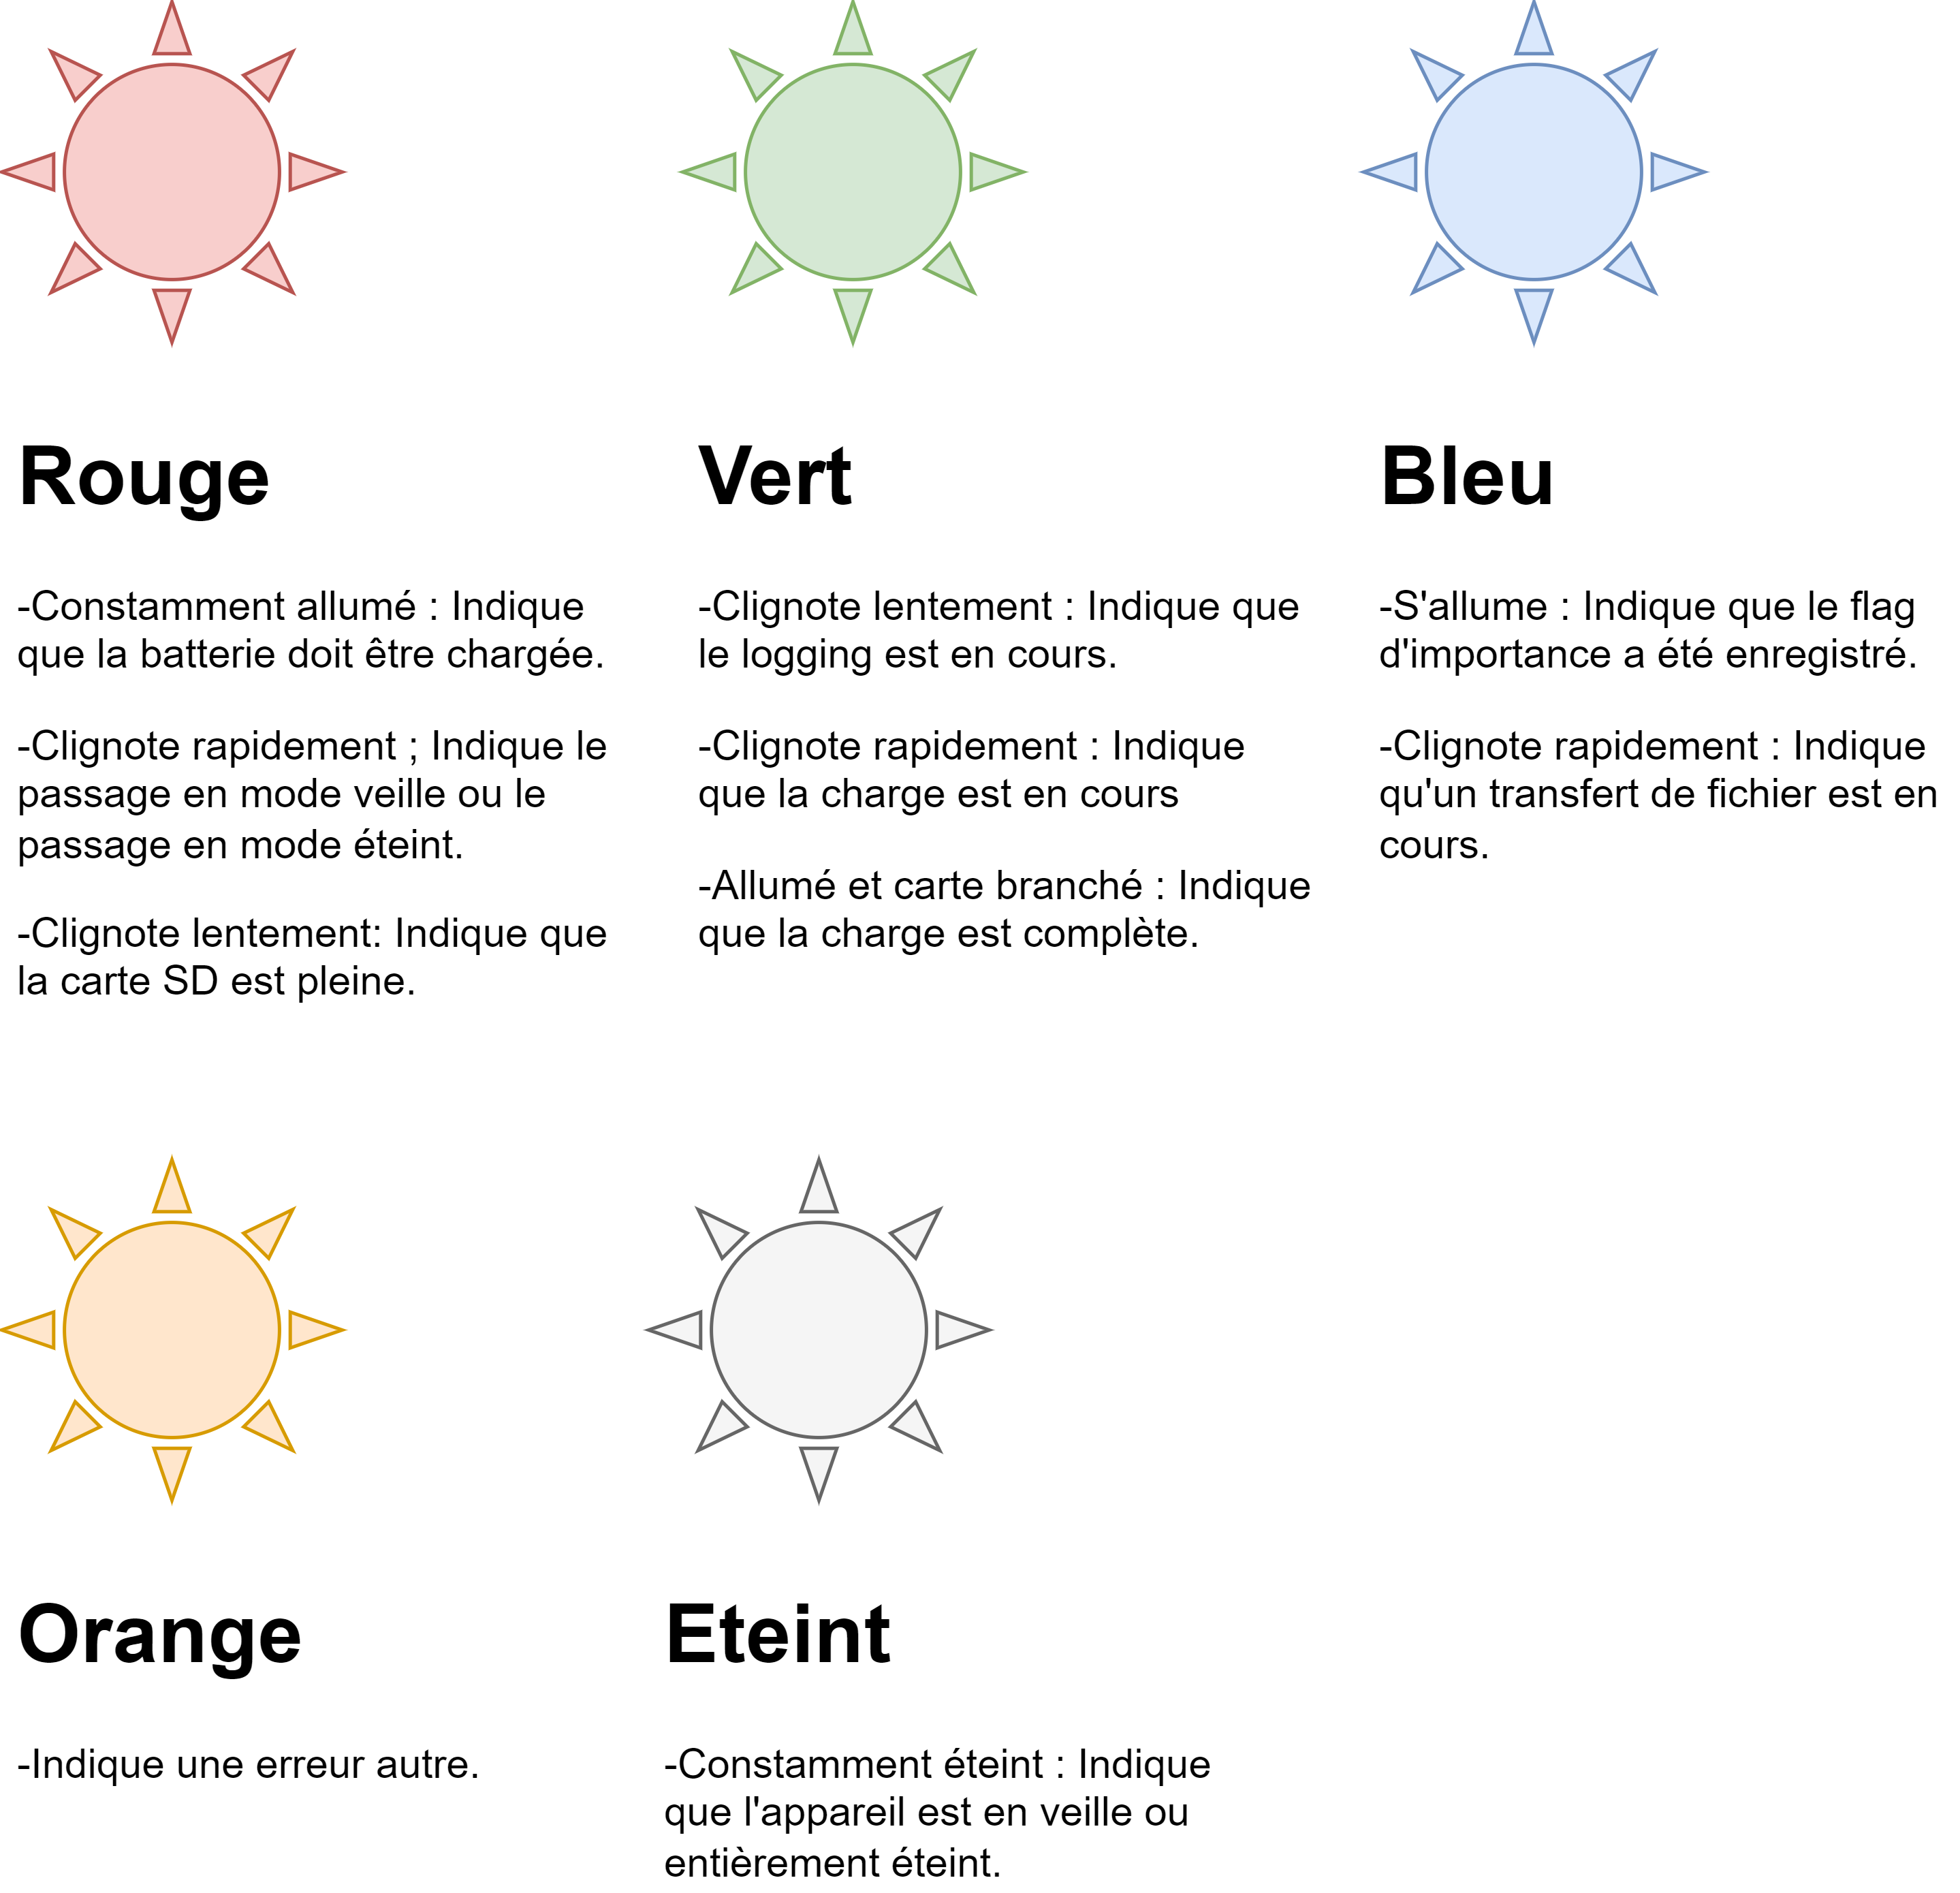
\includegraphics[width=0.55\linewidth]{Images/Dev-SCH/LEDStates}
		\caption{Status LED d'interface}
		\label{fig:ledstates}
	\end{figure}
\end{frame}
	
\begin{frame}[containsverbatim]{Adaptation mécanique}
		\begin{figure}
		\par
		\noindent
		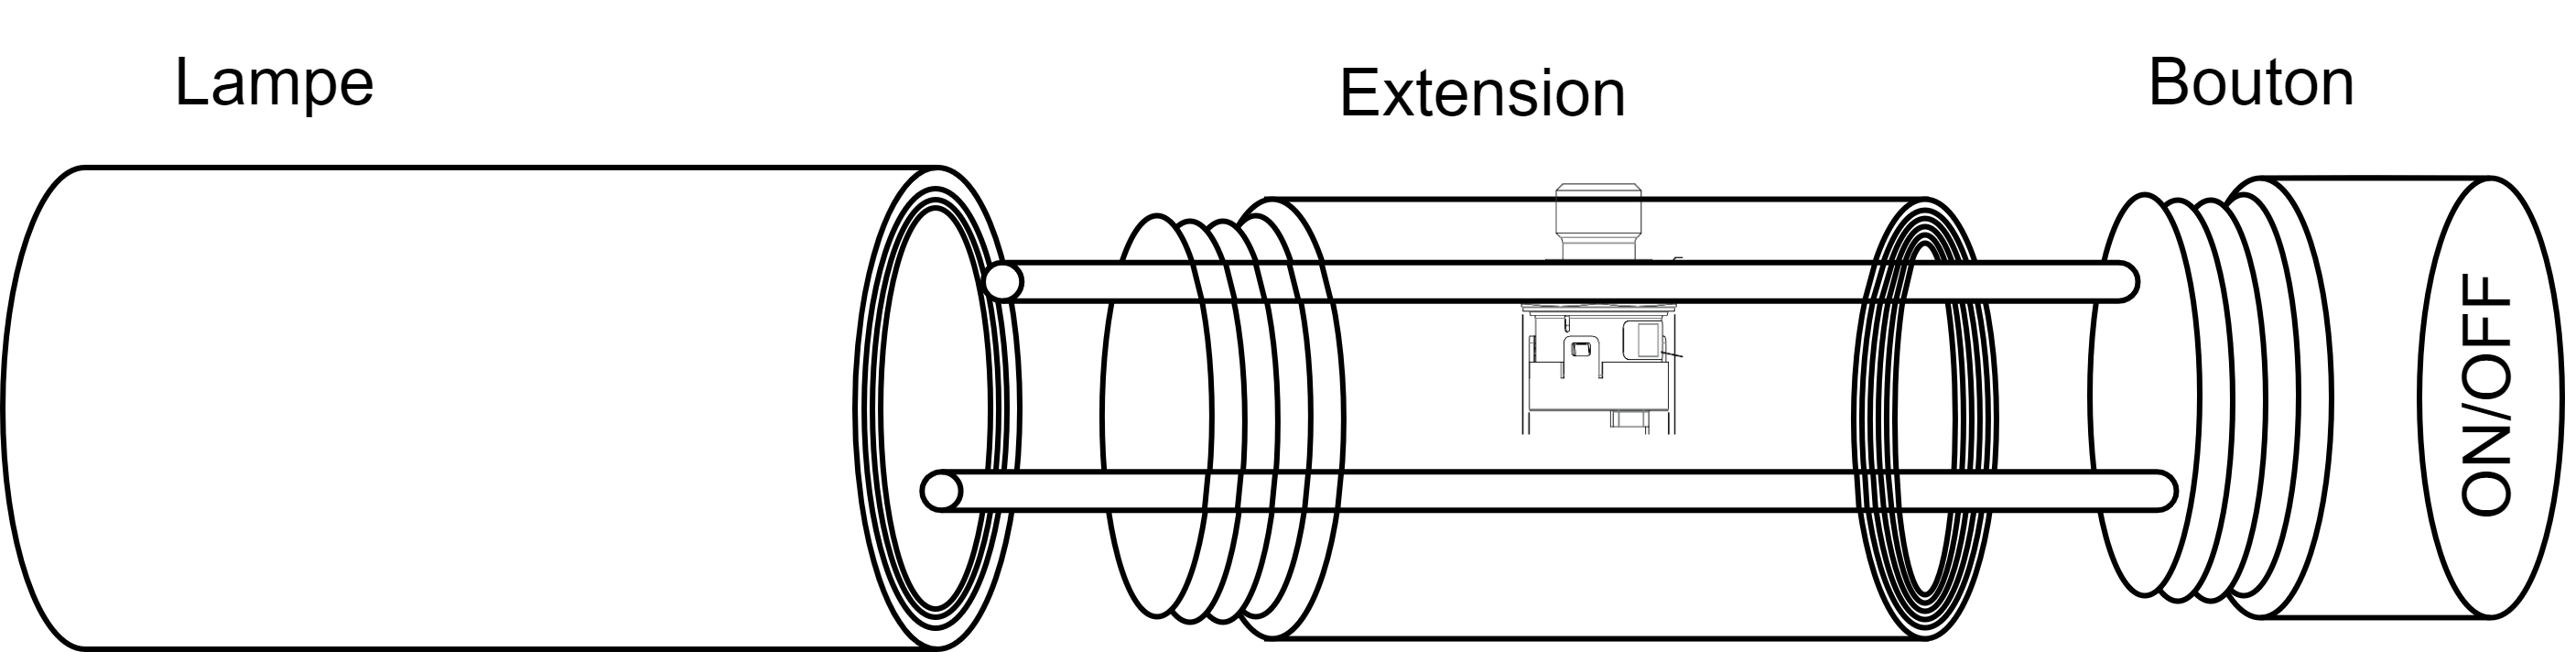
\includegraphics[width=0.7\linewidth]{Images/Dev-SCH/MecaniqueProto2}%
		\hfill
		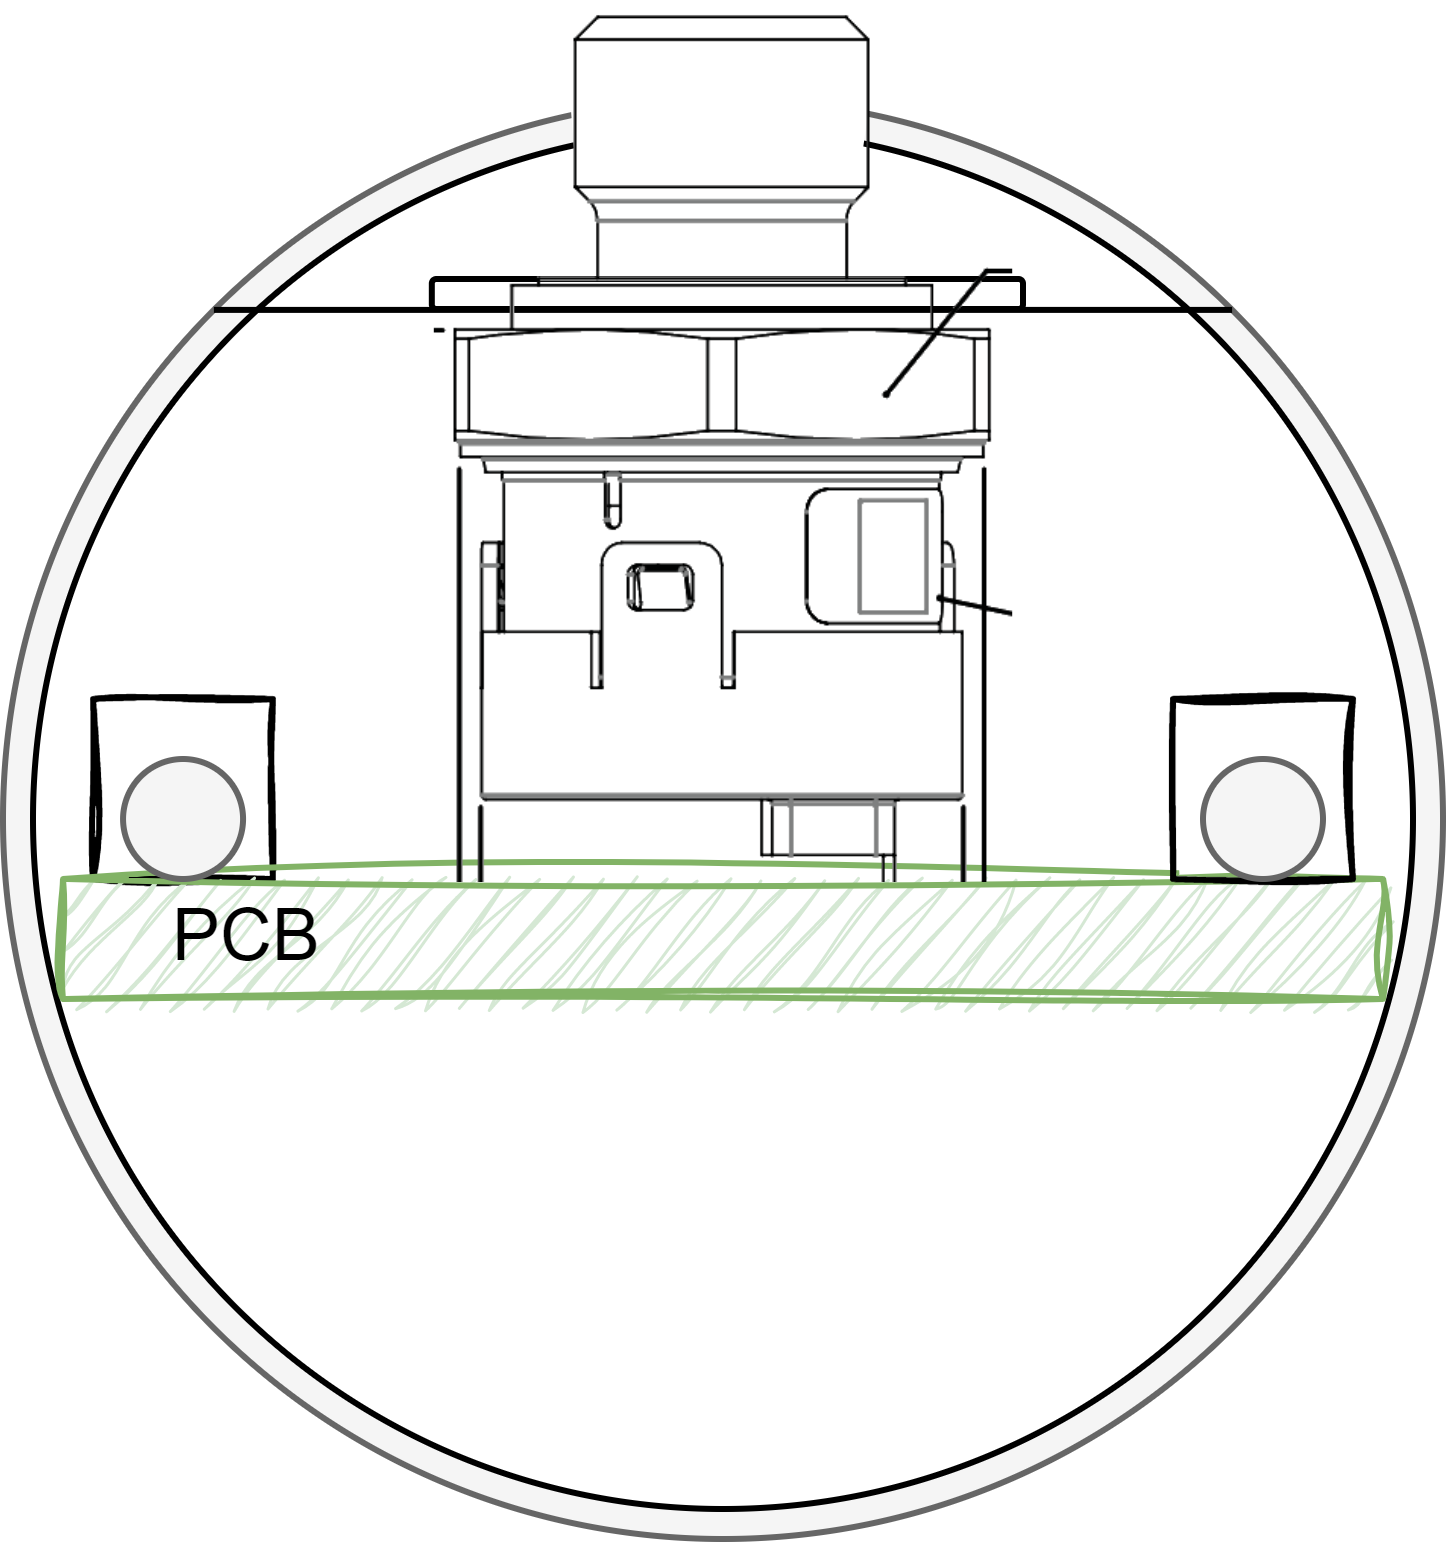
\includegraphics[width=0.25\linewidth]{Images/Dev-SCH/MecaniqueProto1}%
		\par
		\caption{Schéma bloc du système à jour}
	\end{figure}
\end{frame}

\section{Schématique}

\begin{frame}[containsverbatim]{Bus de commutations}
	 \par
	 \noindent
	 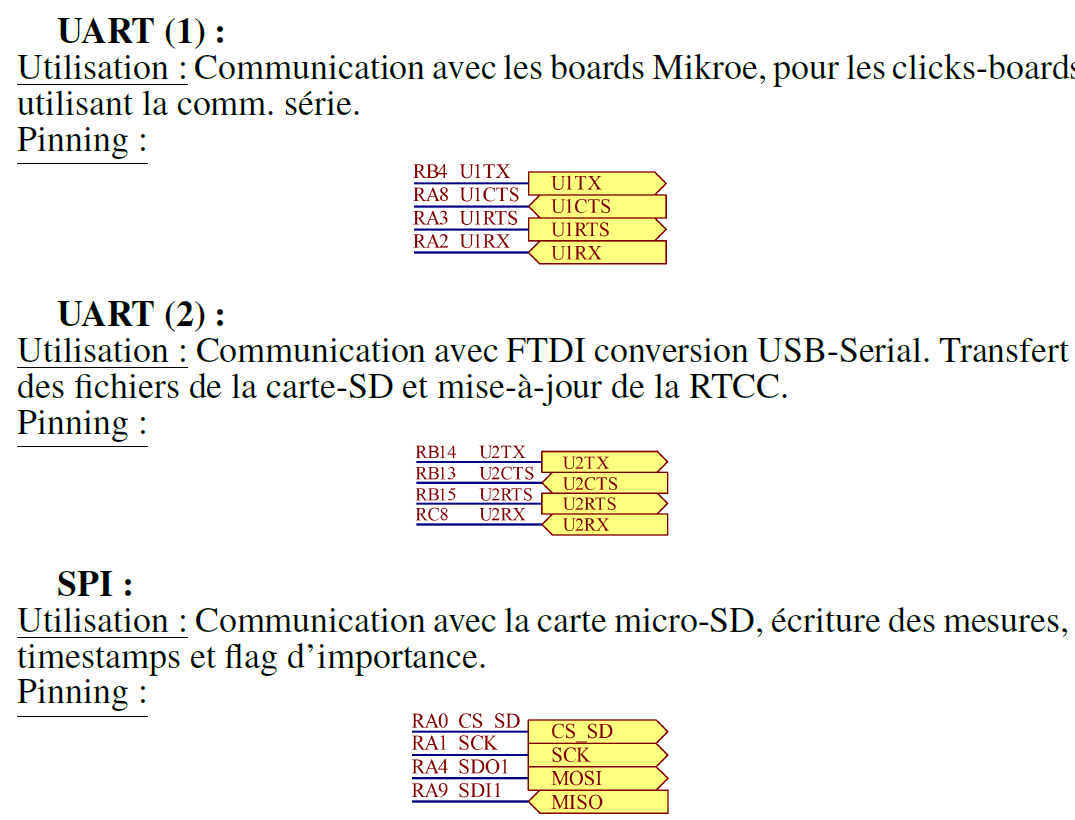
\includegraphics[width=0.49\linewidth]{Images/Dev-SCH/UART12Spi}
	 \hfill
	 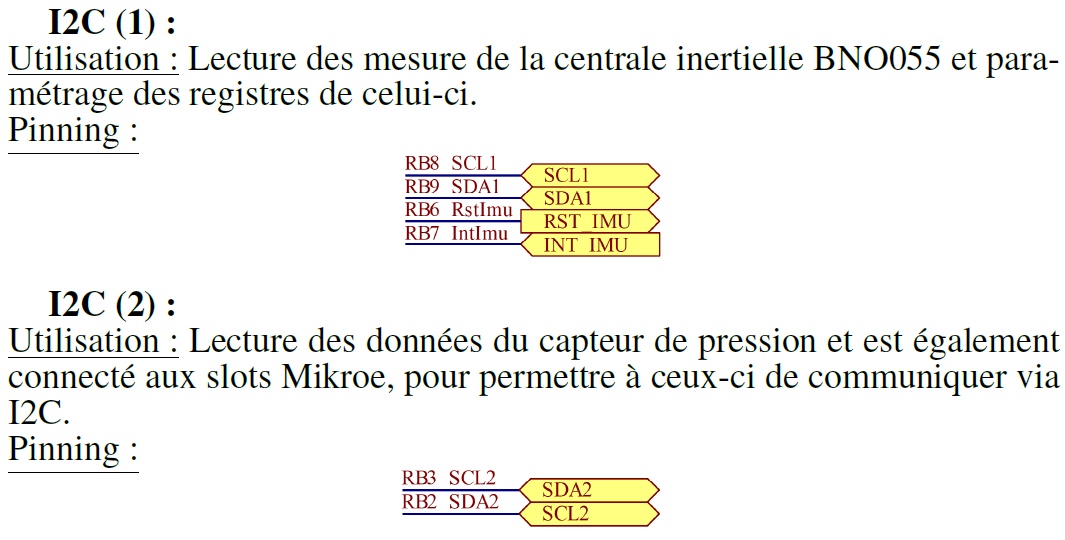
\includegraphics[width=0.49\linewidth]{Images/Dev-SCH/I2C1I2C2}
	 \par	 
\end{frame}

\begin{frame}[containsverbatim]{Périphériques}
	 \par
	\noindent
	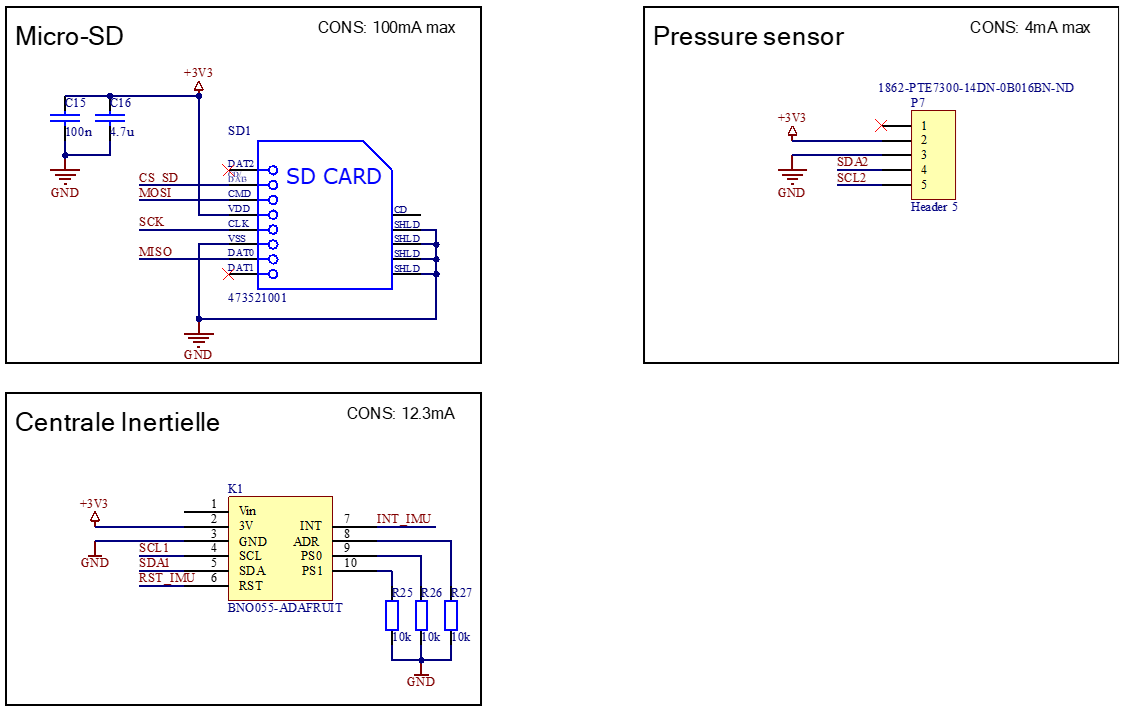
\includegraphics[width=0.49\linewidth]{Images/Dev-SCH/Periph1}
	\hfill
	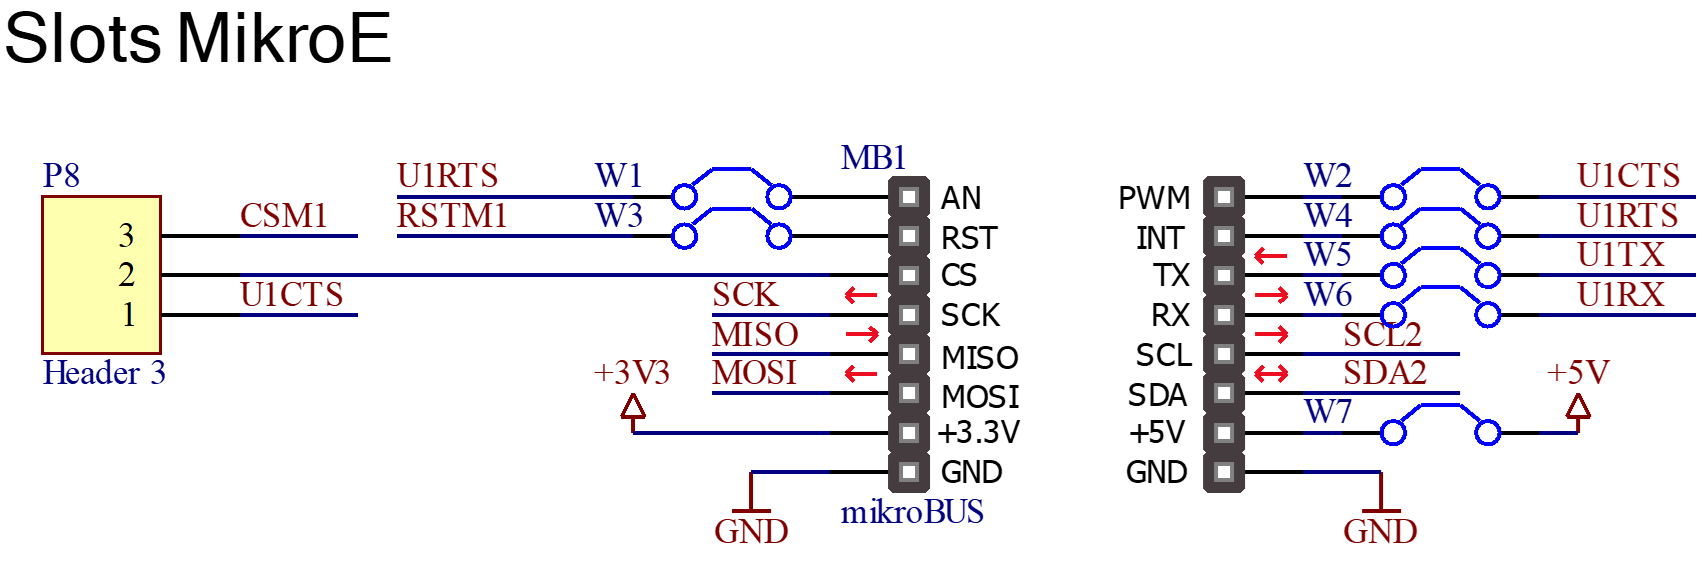
\includegraphics[width=0.49\linewidth]{Images/Dev-SCH/Mikroe}
	\par	 
\end{frame}

\begin{frame}[containsverbatim]{Chargeur de batterie}
	\begin{figure}[h]
		\centering
		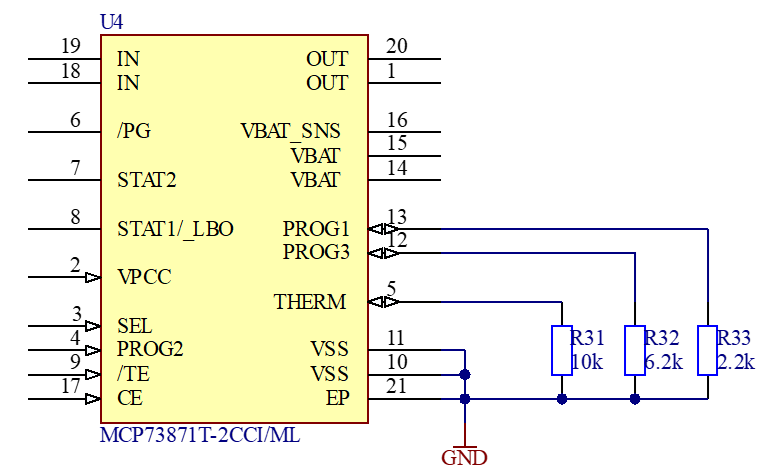
\includegraphics[width=0.3\linewidth]{Images/Dev-SCH/ChargeBat}
	\end{figure}
	$C = 3400mAh$ \quad $ratio_{term} = 0.05$ \quad $ratio_{chrg} = 0.1$\vspace{-2mm}
	\begin{equation} \label{equ:ich}
		I_{term} = C * ratio_{chrg} 
	\end{equation}
	D'après \ref{equ:ich}, $I_{term} = 170mA$.\vspace{-3mm}
	\begin{equation} \label{equ:Rprog3}
		Rprog3 = \frac{1000V}{I_{term}}
	\end{equation}
	$Rprog3 = 5k88 \Omega$ E12 $\Longrightarrow$ $6k2\Omega$.\vspace{-3mm}
	\begin{equation} \label{equ:Rprog1}
		Rprog1 = \frac{1000V}{C * ratio_{chrg}} 
	\end{equation} \vspace{-3mm}
	$Rprog1 = 2k94 \Omega$ E12 $\Longrightarrow$ $2k2\Omega$.
\end{frame}

\begin{frame}[containsverbatim]{Prix des composants}
	\begin{figure}
		\centering
		\label{fig:bomavecprix}
		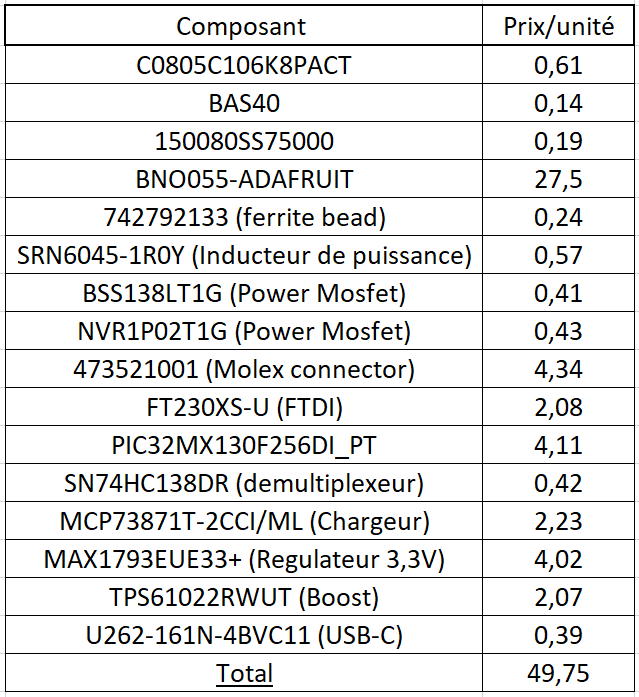
\includegraphics[width=0.45\linewidth]{Images/Dev-SCH/BOMavecPrix}
	\end{figure}
\end{frame}

\section{Conclusion}

\begin{frame}[containsverbatim]{Conclusion et perspectives}
	Lors du développement de la schématique, je n’ai pas eu de grands
	dimensionnements à faire mais plutôt dû mettre en place des mécanismes
	permettant la communication avec tous les senseurs et périphériques du
	système.
	
	Désormais il vas falloir préparer la création du PCB, en contrôlant les
	footprints du circuit et développer d’avantage l’aspect mécanique du projet.
	
	\begin{figure}
		\centering
		\label{fig:lightbulb}
		
\includegraphics[width=0.15\linewidth]{Images/Dev-SCH/lightbulb}
	\end{figure}
	
	
\end{frame}

\section{Questions ?}

\end{document}






